\begin{multicols}{2}
\nolinenumbers
\section{薛定谔方程}
\paragraph{}薛定谔方程在量子力学中占有十分重要的位置,根据量子力学的六个假定,正是薛定谔方程决定了物理体系随时间演变的规律\cite{QUANTUM}。
\begin{tauenv}[frametitle=薛定谔方程]
    \begin{align}
        i\hbar\dv{ }{t}|\varphi(t)\rangle=\hat{H}|\varphi(t)\rangle
    \end{align}
\end{tauenv}
由此可知,只要给出了初态$|\varphi(0)\rangle$就足以决定此后任意时刻的态$|\varphi(t)\rangle$。因此在物理体系演变过程中发没有任何不确定性。
\subsection{原子单位制}
\paragraph{}在数值计算中,一些常数,比如$\hbar,m_e,\varepsilon$等,不仅使得公式非常繁琐,并且在实际的计算当中增加了复杂度,同时由于这些常数往往很大或者很小,大大降低了计算精度,容易出现数值溢出。为此,人们往往使用原子单位制重写方程:\cite{sb}
\begin{tabular}{c|c}
    \toprule
    \multicolumn{2}{c}{原子单位制} \\[2pt]
    \hline
    质量&$m_e=9.1094\times 10^{-31}kg$\\
    电荷&$e=1.6022\times 10^{-19}C$\\
    角动量&$\hbar=1.0546\times 10^{-43}J\cdot s$\\
    介电常数&$4\pi\varepsilon_0=1.1127\times 10^{-10}F\cdot m^{-1}$\\
    长度&$a_0=\frac{4\pi\varepsilon_0\hbar^2}{m_ee^2}=5.2918\times 10^{-11}m$\\
    能量&$Hartree=\frac{m_ee^2}{(4\pi\varepsilon_0)^2\hbar}=4.3597\times 10^{-18}J$\\
    \bottomrule
\end{tabular}
\\
在合适的单位制下(事实上此处也并非原子单位制,而是令$\frac{\hbar^2}{2m}=0$),二维的薛定谔方程改写为:
\begin{equation}
    \begin{gathered}
        i\dv{}{t}|\varphi(t)\rangle=\hat{H}|\varphi(t)\rangle\\
        \hat{H}=-\pdv[2]{}{x}-\pdv[2]{}{y}+V(\mathbf{r})\label{se}
    \end{gathered}
\end{equation}
\section{数值解法}
\subsection{离散化}
显然,数值求解薛定谔方程之前需要对方程\ref{se}进行离散化,设$\delta$为网格的间距,用$\psi_{l,k}(t)$近似地表示$\varphi(l\delta,k\delta,t)$。用最简单的差分近似替代关于x,y的导数:
\begin{align}
    \frac{\partial^2\psi(x,y,t)}{\partial x^2}&\approx \frac{\psi(x+\delta,y,t)-2\psi(x,y,t)+\psi(x-\delta,y,t)}{\delta^2}\\
    &=\delta^{-2}[\psi_{l+1,k}-2\psi_{l,k}+\psi_{l+1,k}]
\end{align}
一维的离散薛定谔方程可以写成
\begin{align*}
    \pdv{\psi(t)}{t}=-i\{-\delta^{-2}[\psi_{l+1}+\psi_{l-1}]+v_{l}\}
\end{align*}
哈密顿量可以写为矩阵的形式
\[ \hat{H} = \left[
\begin{array}{cccc}
v_1 & -\delta^2 & \ldots & 0\\
-\delta^2  & v_1 & \ldots & 0\\
\vdots & \vdots & \ddots & \vdots\\
0 & 0 & \ldots & v_l\\
\end{array} \right] \]
同理,二维的薛定谔方程可以写为\\
\begin{align}
    \pdv{\psi(t)}{t}=-i\{-\delta^{-2}[\psi_{l+1,k}+\psi_{l-1,k}+\psi_{l,k+1}+\psi_{l,k-1}]+v_{l,k}\}
    \label{2d}
\end{align}
其中$v_{l,k}=V(x,y)-4$。如果我们将$\psi_{lk}$按照先排列x方向后y方向的方式堆积成一个列向量,即:
\begin{equation}
    \psi_{lk}=\psi_{n},n=(k-1)L+l
\end{equation},
那么$\hat{H}$仍然可以写成一个矩阵:
\[ \hat{H} = \left[
\begin{array}{cccccc}
v_{11} & -\delta^2  & \cdots &-\delta^2  &\cdots & 0\\
-\delta^2  & v_{12} & \cdots& \cdots & \cdots & 0\\
\vdots & \vdots & \vdots & \vdots& \vdots& \vdots \\
-\delta^2 &0& \cdots &\cdots & \cdots& 0\\
\vdots &\vdots &\vdots & \vdots &  \vdots & \vdots \\
0 & 0 & \cdots & \cdots & -\delta^2  &v_{LK}\\
\end{array} \right] \]
方程\ref{2d}也可以理解为一个粒子在$N=L\times K$的二维网格中传播,这种理解对于处理更加复杂的哈密顿量是十分重要的。
\begin{equation}
    \begin{gathered}
        \hat{H}=-t\sum_{n}^{N}(c^{\dag}_{n+1}c_{n}+c^{\dag}_{n}c_{n+1}+c^{\dag}_{n+L}c_{n}+c^{\dag}_{n}c_{n+L}-W\sum_{n}^{N}\epsilon_nc^{\dag}_nc_n)\\
        |\varphi(t)\rangle=\sum_{n=1}^{N+1}\psi_n(t)c^{\dag}_n|0\rangle
    \end{gathered}
    \label{cc}
\end{equation}
$c^{\dag},c$是产生湮灭算符。对比方程\ref{2d}和\ref{cc},不难发现$t=\delta^{-2},W\epsilon_n=v_n$。
\subsection{矩阵指数}
与普通的微分方程类似,矩阵微分方程有解析解\cite{De1996}:
\begin{equation}
    \begin{aligned}
        i\dv{\hat{U}(t)}{t}=\hat{H}(t)\hat{U}\\
        \hat{U}(t)=e^{-i\hat{H}t}\hat{U}(0)
    \end{aligned}
\end{equation}
问题的关键在于求出$e^{-i\hat{H}t}$。矩阵指数由Taylor级数定义:
\begin{align}
    e^{xH}=\sum_{n=0}^{\infty}\frac{x^n}{n!}H^n
\end{align}
尽管这样的展开在数学上是非常重要的,但是在实际计算中没有意义,一方面存储矩阵需要占用大量的内存,对计算资源造成巨大的浪费;另一方面,Taylor展开无法满足波函数模方守恒的要求:
\begin{equation}
    \begin{aligned}
        &\langle \varphi(0)|\varphi(0)\rangle=\langle \varphi(t)|\varphi(t)\rangle\\
        &\neq\langle\varphi(0)|(I+itH-\frac{t^2}{2}H+\cdots)(I-itH-\frac{t^2}{2}H+\cdots)|\varphi(0)\rangle
    \end{aligned}
\end{equation}
为此我们引入切比雪夫多项式方法计算$e^{-i\hat{H}t}$
\subsection{切比雪夫多项式}
为了演化波函数,需要对时间演化算子进行数值展开,由于哈密顿量是稀疏的,所以可以方便地使用Chebyshev多项式进行展开,这种方法对求解含时薛定谔方程是无条件稳定的。假设$x\in[-1,1]$,
\begin{equation}
    e^{-izx}=J_0(z)+2\sum_{m=1}^{\infty}(-i)^mJ_m(z)T_m(x)
\end{equation}
其中$J_m$是m阶贝塞尔函数,$T_m$是第一类切比雪夫多项式。$T_m(x)$可以由递归关系求解:
\begin{equation}
    T_{m+1}(x)=2xT_{m}-T_{m-1}
\end{equation}
为了利用切比雪夫多项式方法,我们需要将$\hat{H}$缩放为$\tilde{H}=\hat{H}\Vert H\Vert$,使$\tilde{H}$的特征值分布在$[-1,1]$。
\begin{equation}
    |\varphi(t)\rangle=\{J_0(\tau)+2\sum_{m=1}^{\infty}(-i)^mJ_m(\tau)\hat{T}_m(\tilde{H})\}|\varphi(0)\rangle
\end{equation}
$\tau=t\cdot\Vert H\Vert$。在实际计算中不需要存储$\hat{T}_m$,而是由递归关系直接计算波函数:
\begin{equation}
    \hat{T}_{m+1}(\tilde{H})\varphi(0)=2\tilde{H}\hat{T}_{m}(\tilde{H})\varphi(0)-\hat{T}_{m-1}(\tilde{H})\varphi(0)
\end{equation}
除了时间演化算子$e^{-it\hat{H}}$外,其他算子也可以使用类似方法,展开为切比雪夫多项式的级数。
\begin{equation}
    f(x)=\frac{1}{2}c_0T_0(x)+\sum_{m}c_mT_m(x)
\end{equation}
系数定义为
\begin{equation}
    c_m=\frac{2}{\pi}\int_{-1}^{1}\frac{\dd{x}}{\sqrt{1-x^2}}f(x)T_m(x)
\end{equation}
令$x=\cos{\theta}$,并带入上式,可以得到:
\begin{equation}
    \begin{aligned}
        c_m=\frac{2}{\pi}\int_{0}^{\pi}f(\cos{\theta})\cos(m\theta)\dd{\theta}\\
        =Re[\frac{2}{\pi}\sum_{n=0}^{N-1}f(\cos\frac{2\pi n}{N})e^{i\frac{2\pi n}{N}m}]
    \end{aligned}
\end{equation}
因此可以使用快速傅里叶变换计算出$c_k$。以Fermi-Dirac算符为例:
\begin{equation}
    \begin{aligned}
        f(\hat{H})&=\frac{ze^{-\beta\hat{H}}}{1+ze^{-\beta\hat{H}}},\\
        \text{where}\quad\beta&=\frac{1}{k_BT},z=e^{\beta\mu}
    \end{aligned}
\end{equation}
我们定义$\tilde{\beta}=\beta\cdot\Vert\hat{H}\Vert$。根据前面的讨论:
\begin{equation}
    f(\tilde{H})=\sum_{m=0}^{\infty}c_mT_m(\tilde{H})
\end{equation}
\section{高斯波包}
\subsection{Theory}
本节我们将用上面提到的方法计算一个高斯波包通过波导时波函数随时间的演化。初始的波函数设置为:
\begin{align}
    \Psi(x,y,t_0)=Ae^{-\frac{x^2}{4\sigma _x^2}-\frac{y^2}{4\sigma _y^2}+ik_0x}
\end{align}
为了合理地设置网格数量和演化时间等参数,我们有必要讨论一个波包自由传播时的解析理论。为简单起见,我们首先考虑一维的情形:
\begin{equation}
    \Psi(x,0)=Ae^{-\frac{x^2}{4\sigma^2}+ik_0x}
\end{equation}
由归一化求得$A=(\frac{1}{2\pi\sigma^2})^\frac{1}{4}$叠加原理告诉我们,自由粒子的波函数时各种波矢的平面波的叠加:
\begin{equation}
    \Psi(x,t)=\frac{1}{\sqrt{2\pi}}\int_{-\infty}^{\infty}g(k)e^{i(kx-\omega t)}dk
\end{equation}
我们已知t=0时刻的波函数,于是可以由傅里叶变换求出$g(k)$:
\begin{equation}
    \begin{aligned}
        g(k)&=\frac{1}{\sqrt{2\pi}}\int \Psi(x,0)e^{-ikx}\dd{dx}\\
        &\frac{A}{\sqrt{2\pi}}\int e^{-\frac{x^2}{4\sigma^2}e^{-i(k-k_0)x}\dd{x}}\\
        &\frac{A}{\sqrt{2\pi}}\int e^{-\frac{1}{(2\sigma)^2}(x+2i(k-k_0)\sigma^2)^2-(k-k_0)^2\sigma^2}\dd{x}
    \end{aligned}
\end{equation}
利用留数的性质可以证明,若满足$-\frac{\pi}{4}<Arg(\alpha)<\frac{\pi}{4}$:
\begin{equation}
    \begin{aligned}
        I(\alpha,\beta)&=\int_{-\infty}^{\infty}e^{-\alpha^2(\xi+\beta)^2}\dd{\xi}\\
        &=I(\alpha,0)=\frac{\sqrt{\pi}}{\alpha}
    \end{aligned}
\end{equation}
于是:
\begin{equation}
    \Psi(x,t)=\frac{\sqrt{2\sigma}}{(2\pi)^{3/4}}\int_{-\infty}^{\infty}e^{-(k-k_0)^2\sigma^2}e^{ikx}\dd{k}
\end{equation}
不难证明t时刻波包的形状仍然为高斯波包。再来计算t时刻波函数的模方:
\begin{equation}
    |\Psi(x,t)|^2=\sqrt{\frac{2}{\pi a^2}}\frac{1}{\sqrt{1+\frac{4\hbar^2t^2}{m^2a^4}}}\exp\{-\frac{2a^2(x-\frac{\hbar k_0t}{m})^2}{a^4+\frac{4\hbar^2t^2}{m^2}}\}
\end{equation}
$a=2\sigma$。此时波包的最大值位于$x_M$:
\begin{equation}
    x_M=\frac{\hbar k_0}{m}t
\end{equation}
求出波包的群速度:
\begin{equation}
    V_G=\dv{x_M}{t}=\frac{\hbar k_0}{m}
\end{equation}
二维波包穿过狭缝时衍射波的角宽度近似满足:
\begin{equation}
    2\theta\approx\frac{2\lambda}{\Delta y}
\end{equation}
\end{multicols}
\subsection{Result}
\begin{figure*}[h!]
    \centering
    \begin{subfigure}{0.3\linewidth}
        \includegraphics[width=\linewidth]{10/0}
    \end{subfigure}
    \begin{subfigure}{0.3\linewidth}
        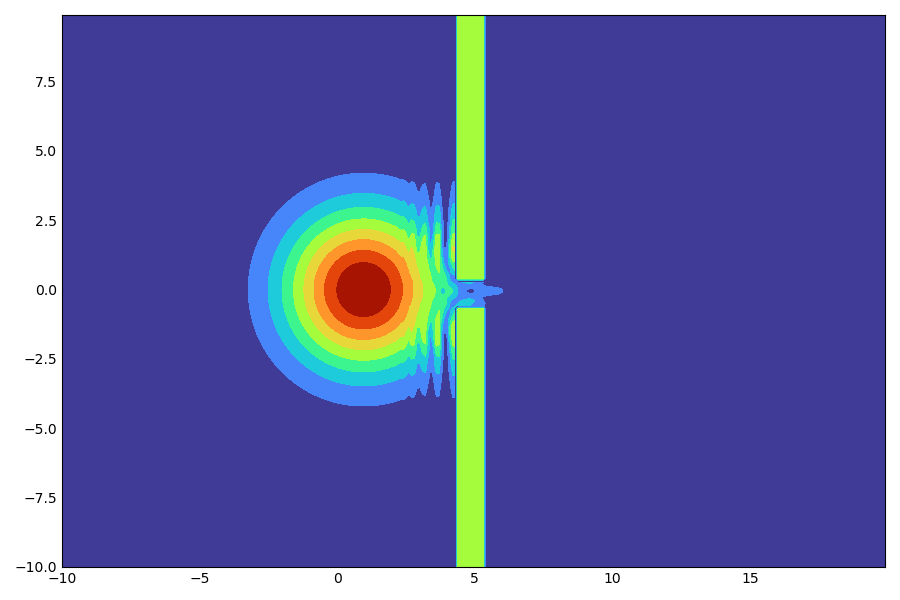
\includegraphics[width=\linewidth]{10/100}
    \end{subfigure}
    \begin{subfigure}{0.3\linewidth}
        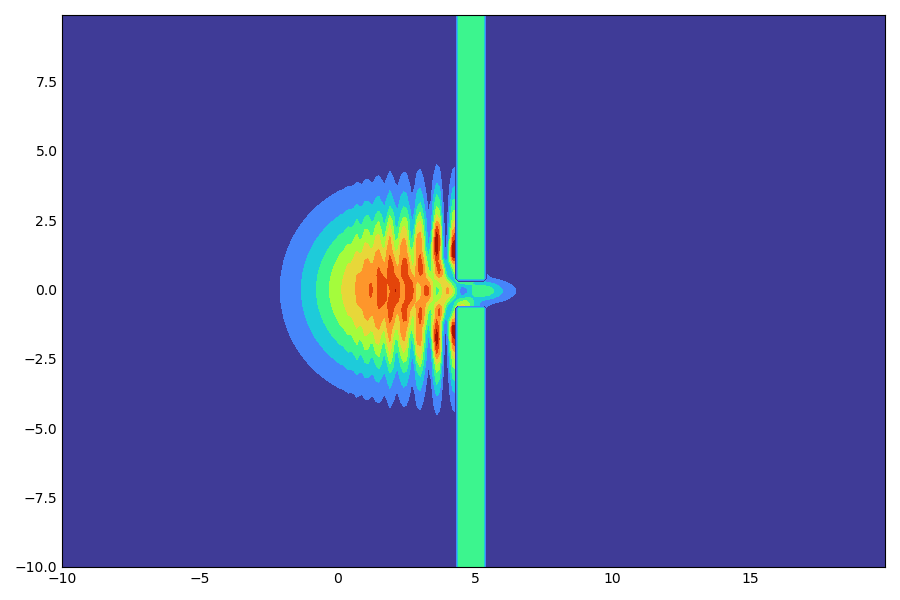
\includegraphics[width=\linewidth]{10/200}
    \end{subfigure}
    \begin{subfigure}{0.3\linewidth}
        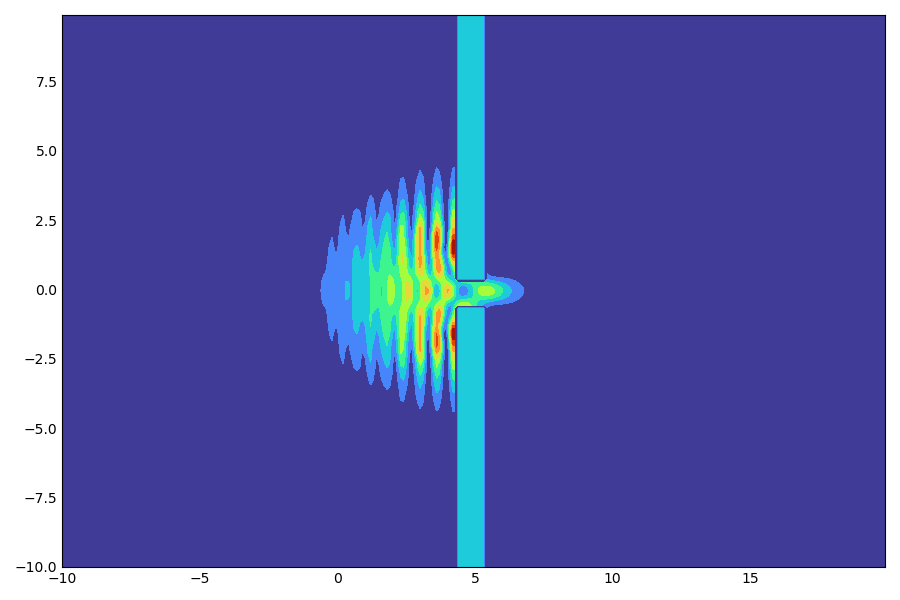
\includegraphics[width=\linewidth]{10/300}
    \end{subfigure}
    \begin{subfigure}{0.3\linewidth}
        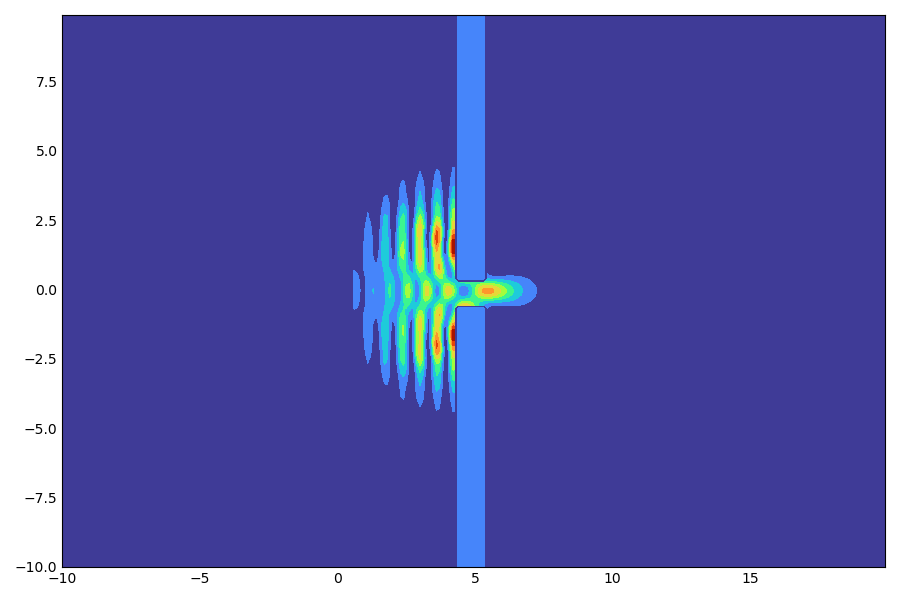
\includegraphics[width=\linewidth]{10/400}
    \end{subfigure}
    \begin{subfigure}{0.3\linewidth}
        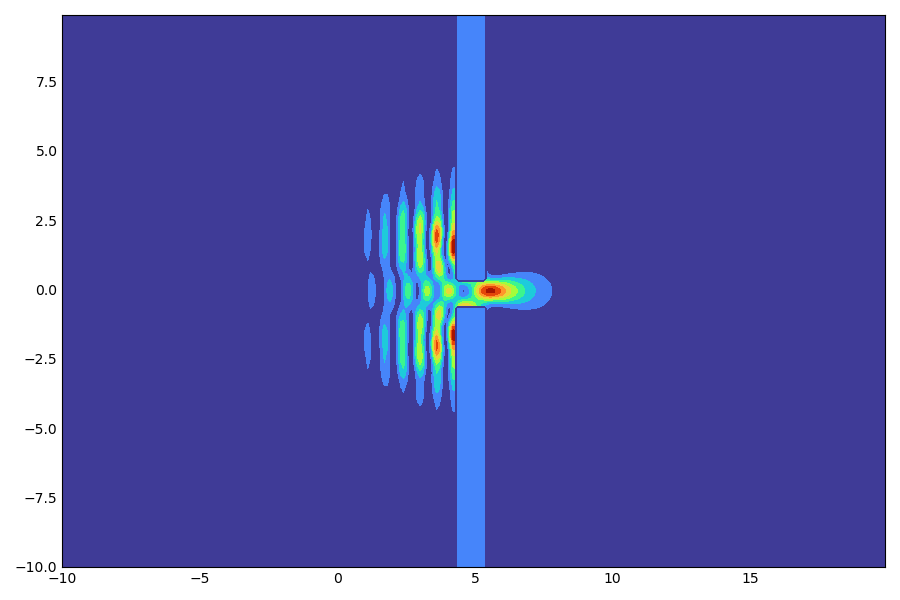
\includegraphics[width=\linewidth]{10/500}
    \end{subfigure}
    \begin{subfigure}{0.3\linewidth}
        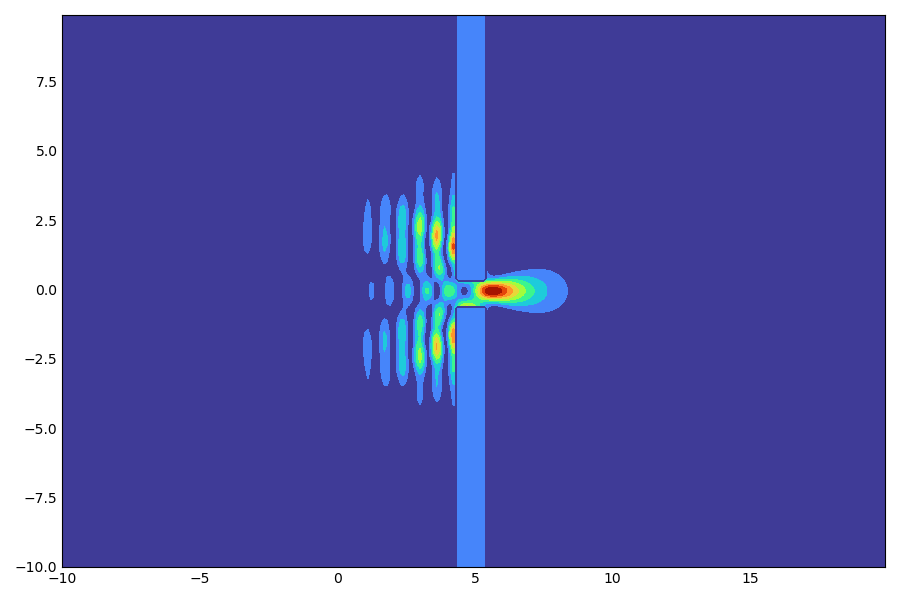
\includegraphics[width=\linewidth]{10/600}
    \end{subfigure}
    \begin{subfigure}{0.3\linewidth}
        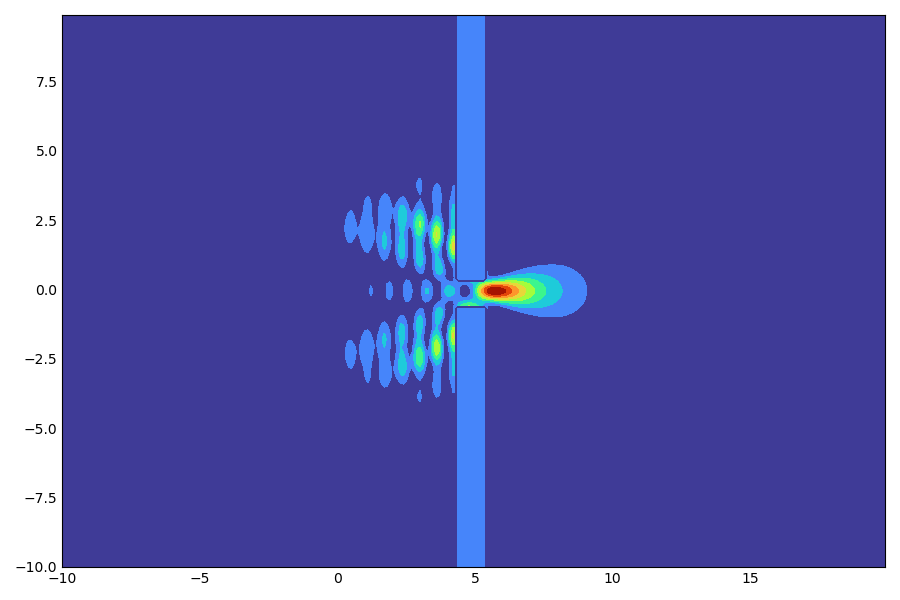
\includegraphics[width=\linewidth]{10/700}
    \end{subfigure}
    \begin{subfigure}{0.3\linewidth}
        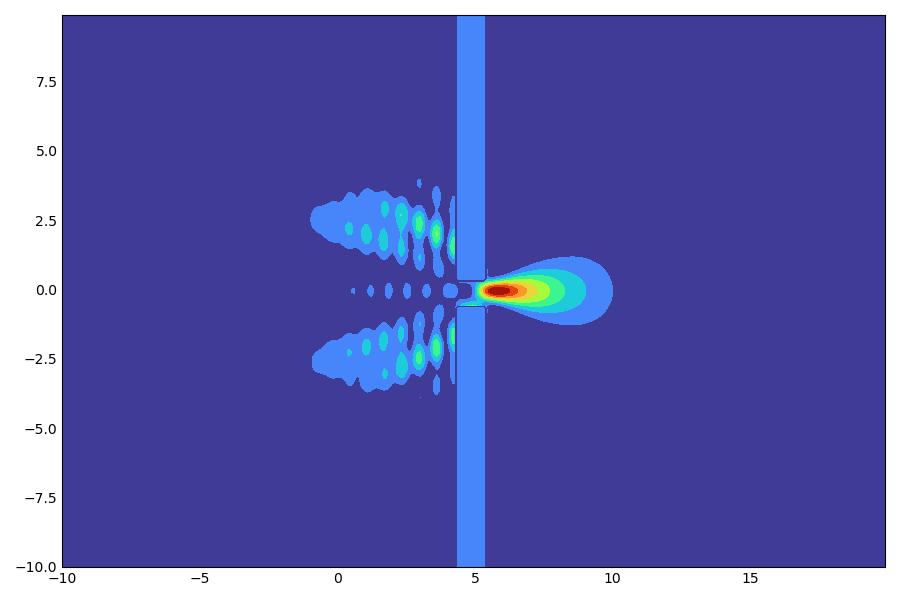
\includegraphics[width=\linewidth]{10/800}
    \end{subfigure}
    \begin{subfigure}{0.3\linewidth}
        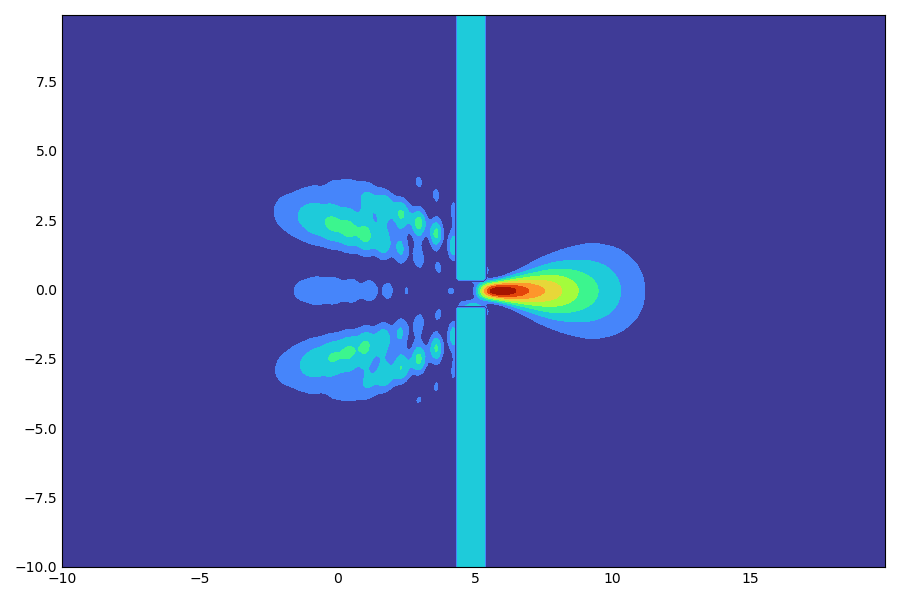
\includegraphics[width=\linewidth]{10/900}
    \end{subfigure}
    \begin{subfigure}{0.3\linewidth}
        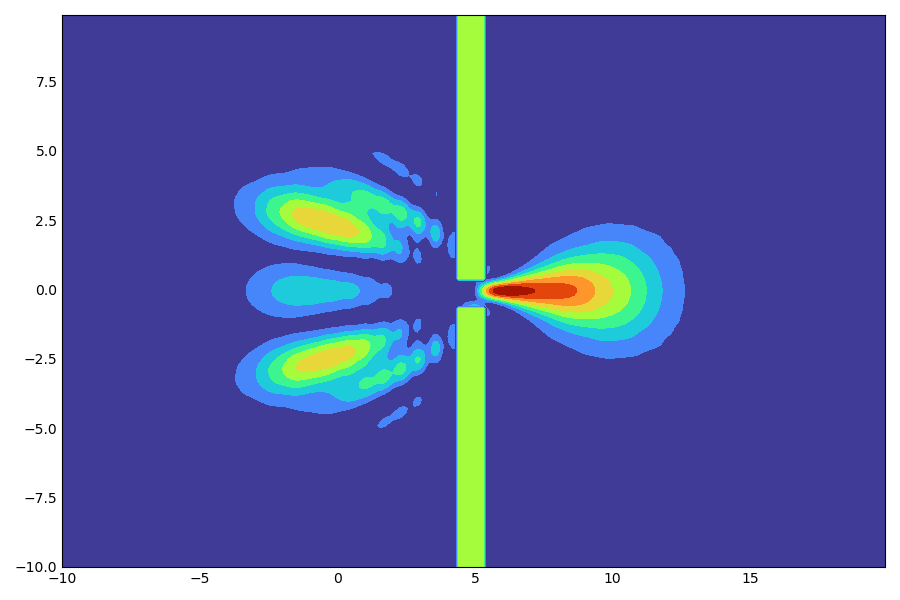
\includegraphics[width=\linewidth]{10/1000}
    \end{subfigure}
    \begin{subfigure}{0.3\linewidth}
        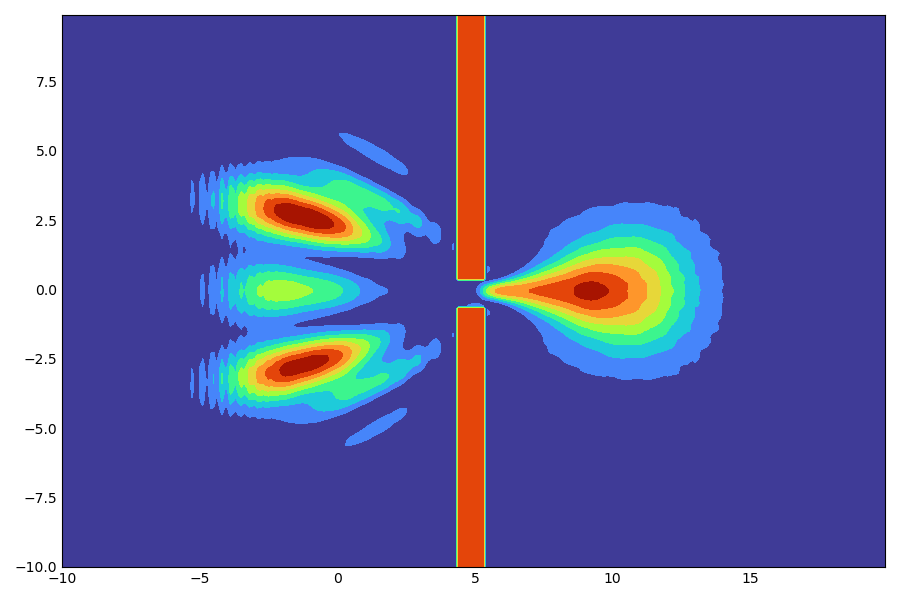
\includegraphics[width=\linewidth]{10/1100}
    \end{subfigure}
    \caption{$\Delta y=20\delta,t\in[0,1100]$}
\end{figure*}
\begin{figure*}[h]
    \centering
    \begin{subfigure}{0.3\linewidth}
        \includegraphics[width=\linewidth]{5/0}
    \end{subfigure}
    \begin{subfigure}{0.3\linewidth}
        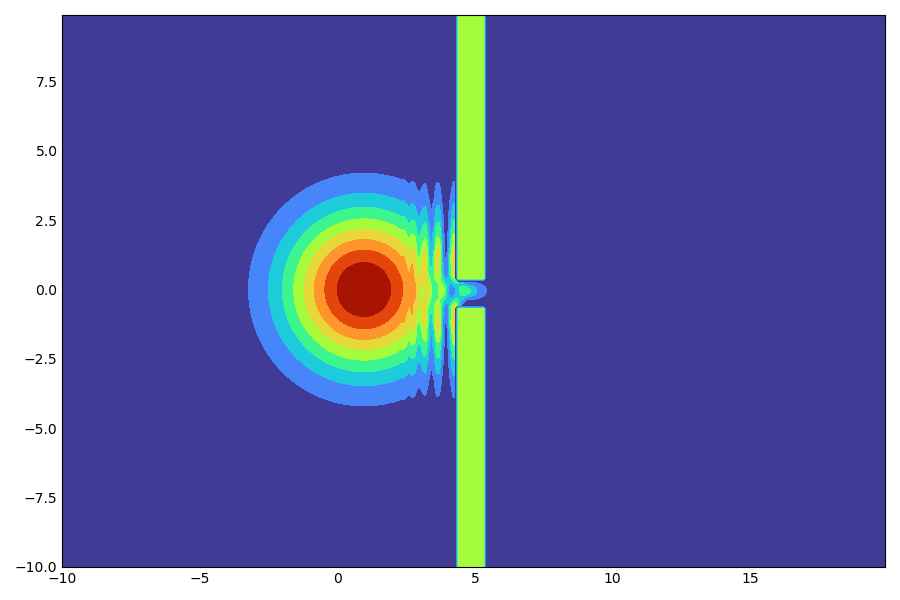
\includegraphics[width=\linewidth]{5/100}
    \end{subfigure}
    \begin{subfigure}{0.3\linewidth}
        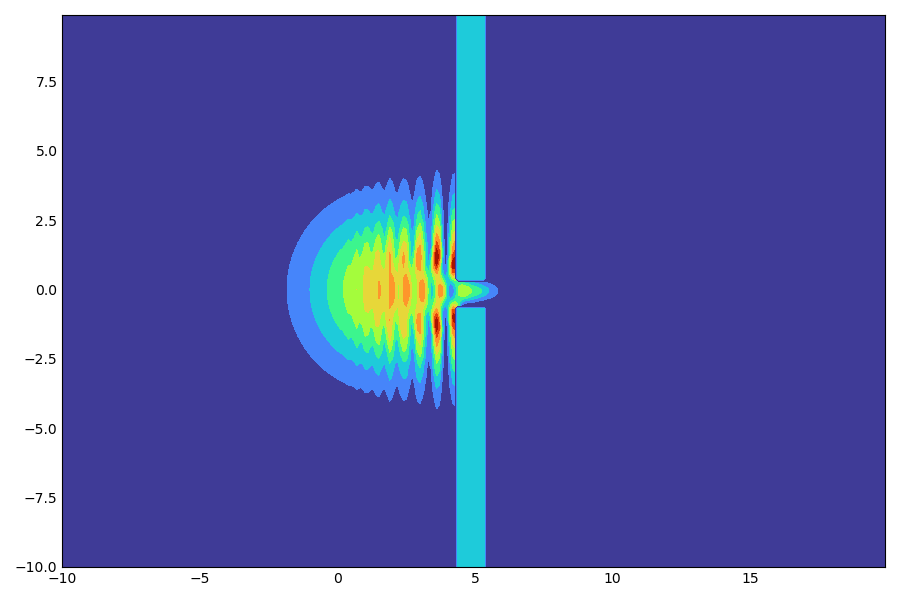
\includegraphics[width=\linewidth]{5/200}
    \end{subfigure}
    \begin{subfigure}{0.3\linewidth}
        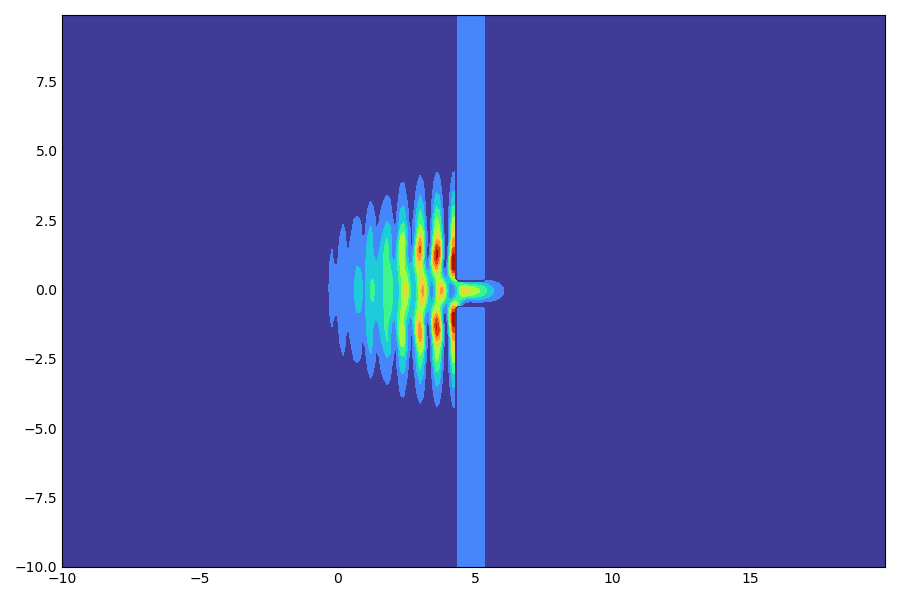
\includegraphics[width=\linewidth]{5/300}
    \end{subfigure}
    \begin{subfigure}{0.3\linewidth}
        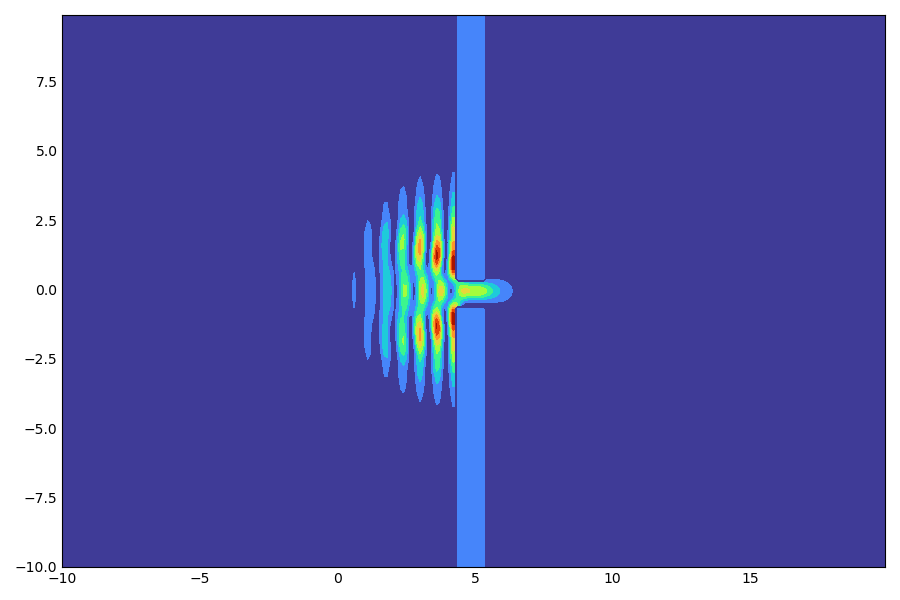
\includegraphics[width=\linewidth]{5/400}
    \end{subfigure}
    \begin{subfigure}{0.3\linewidth}
        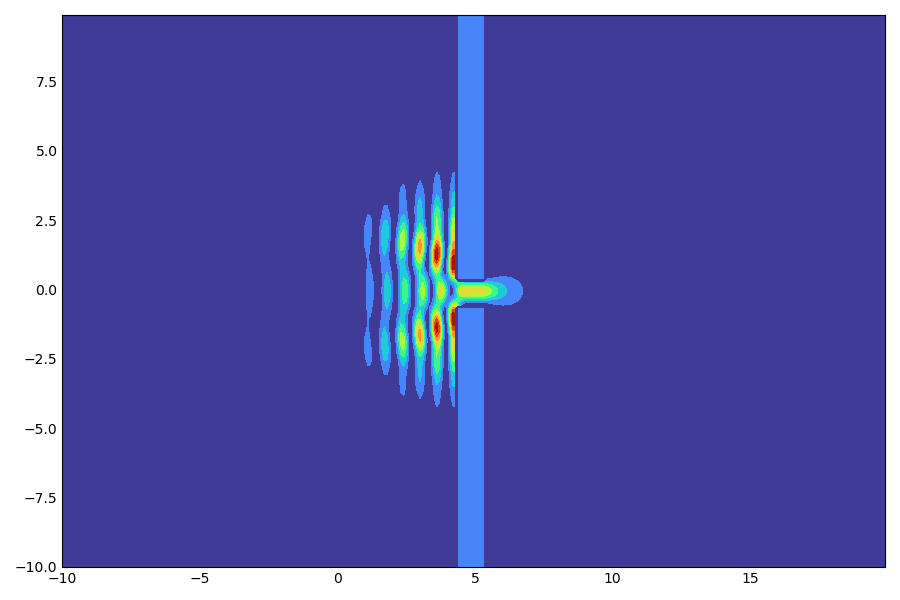
\includegraphics[width=\linewidth]{5/500}
    \end{subfigure}
    \begin{subfigure}{0.3\linewidth}
        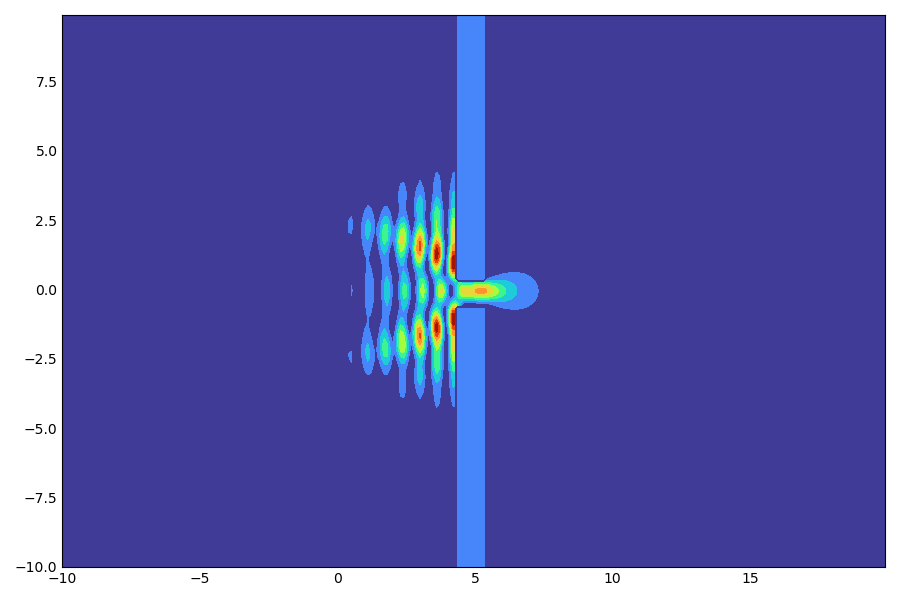
\includegraphics[width=\linewidth]{5/600}
    \end{subfigure}
    \begin{subfigure}{0.3\linewidth}
        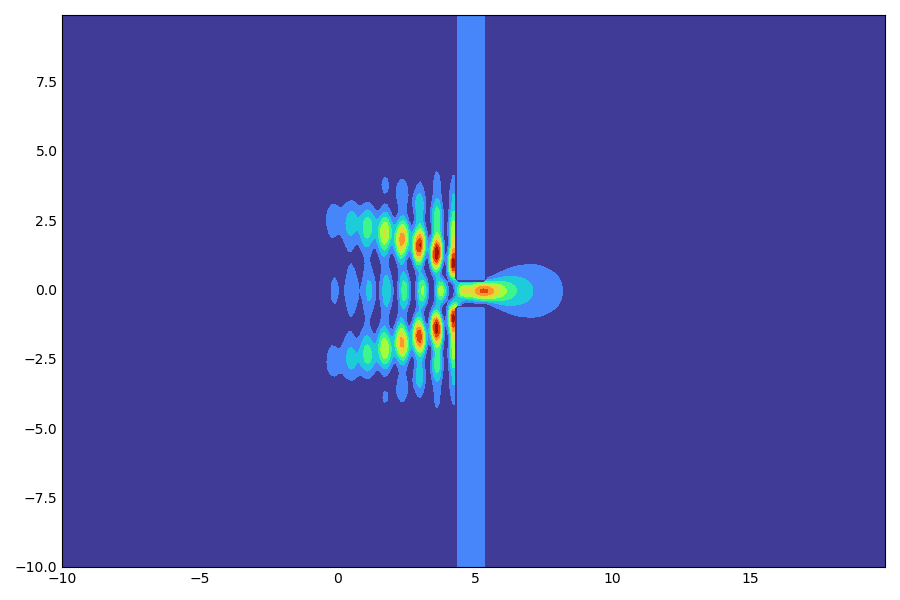
\includegraphics[width=\linewidth]{5/700}
    \end{subfigure}
    \begin{subfigure}{0.3\linewidth}
        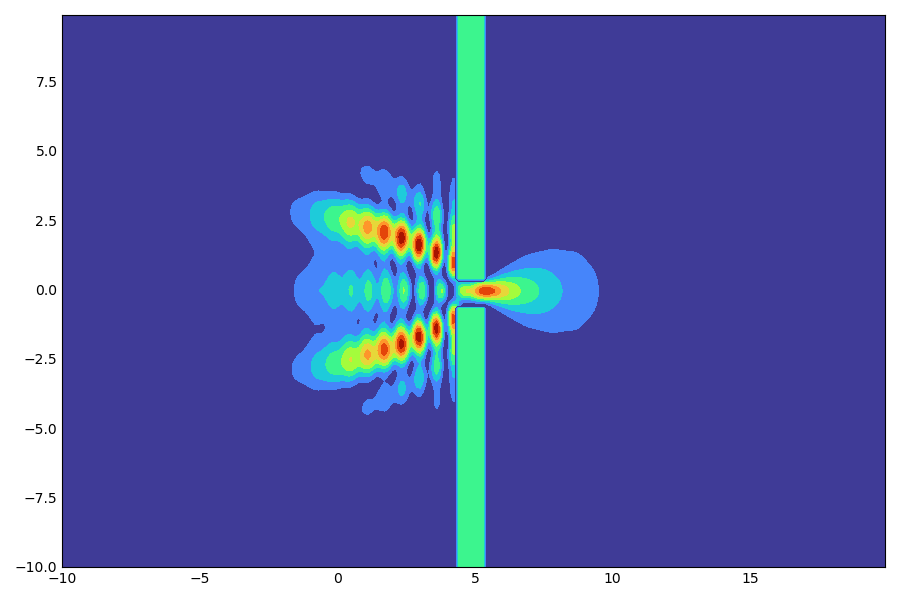
\includegraphics[width=\linewidth]{5/800}
    \end{subfigure}
    \begin{subfigure}{0.3\linewidth}
        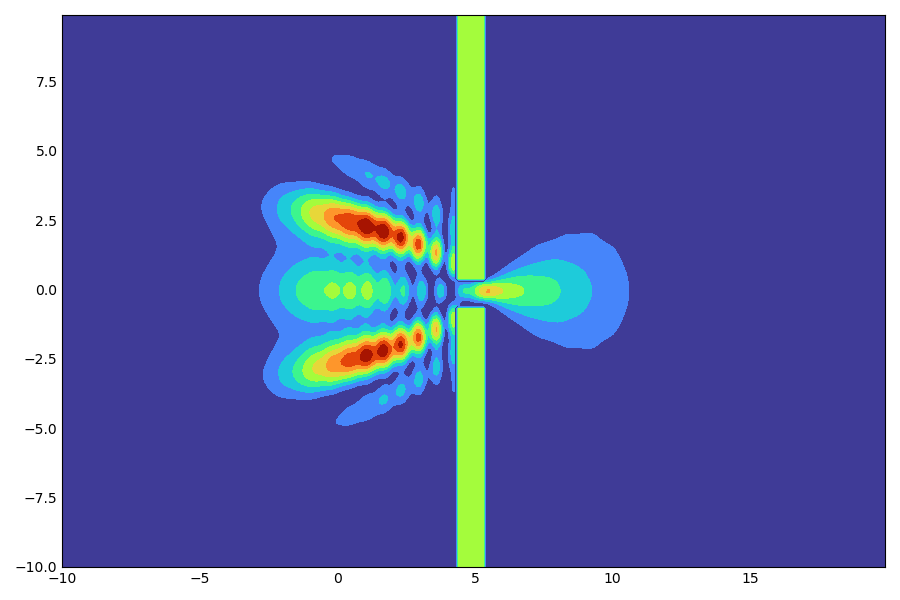
\includegraphics[width=\linewidth]{5/900}
    \end{subfigure}
    \begin{subfigure}{0.3\linewidth}
        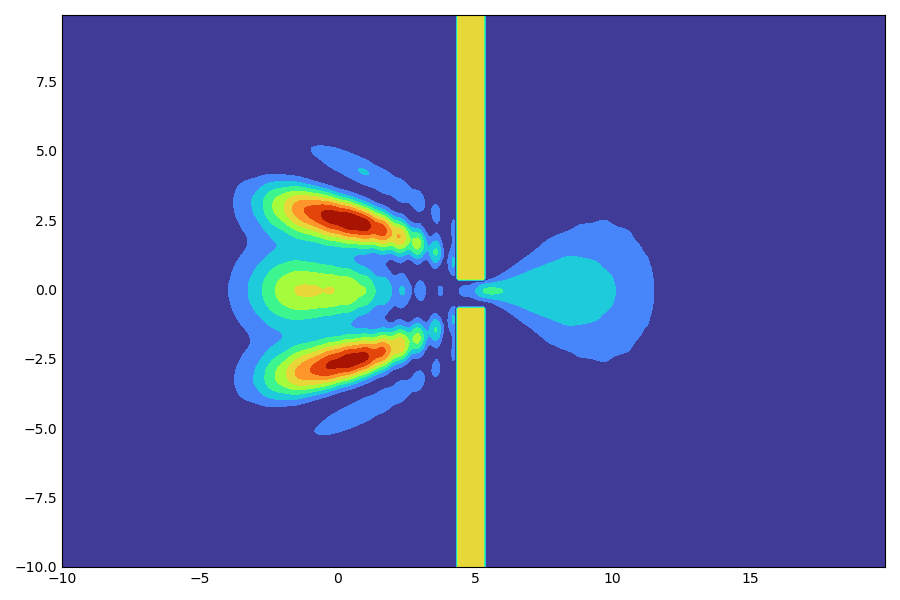
\includegraphics[width=\linewidth]{5/1000}
    \end{subfigure}
    \begin{subfigure}{0.3\linewidth}
        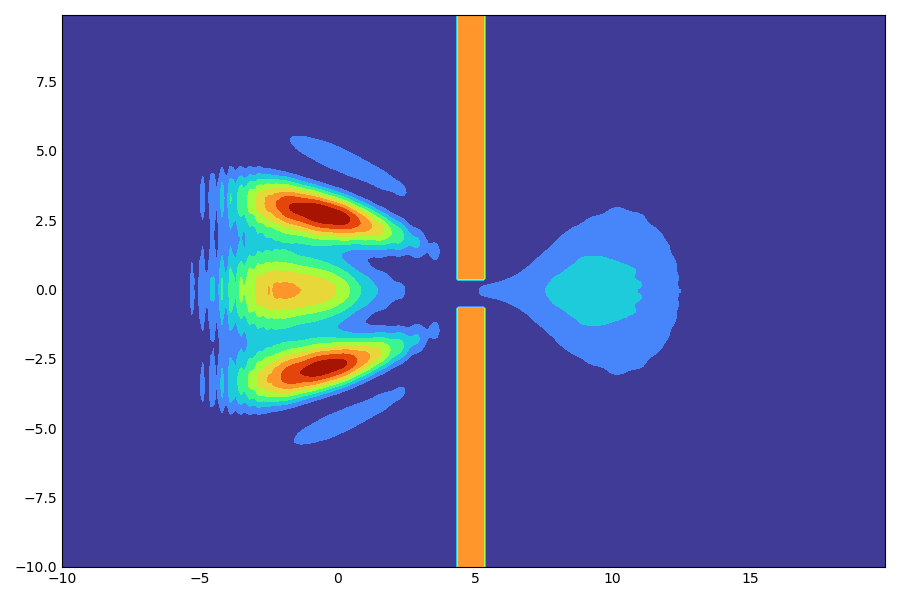
\includegraphics[width=\linewidth]{5/1100}
    \end{subfigure}
    \caption{$\Delta y=10\delta,t\in[0,1100]$}
\end{figure*}
\begin{figure*}[h]
    \centering
    \begin{subfigure}{0.3\linewidth}
        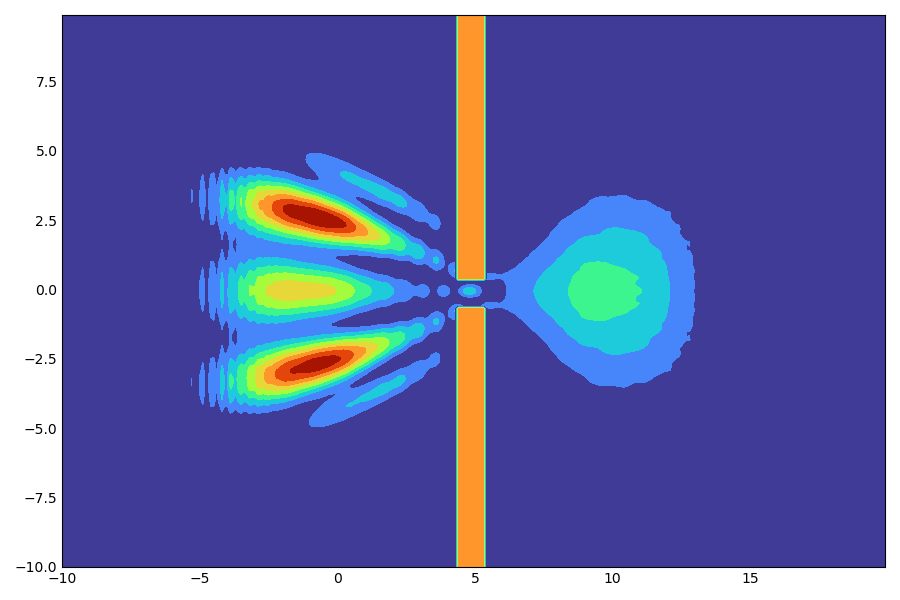
\includegraphics[width=\linewidth]{5/8}
    \end{subfigure}
    \begin{subfigure}{0.3\linewidth}
        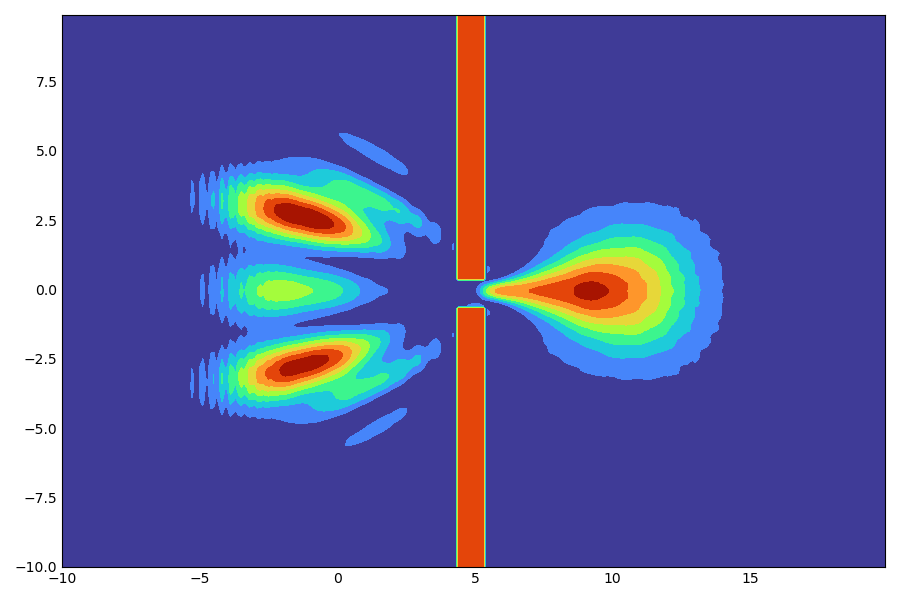
\includegraphics[width=\linewidth]{5/10}
    \end{subfigure}
    \begin{subfigure}{0.3\linewidth}
        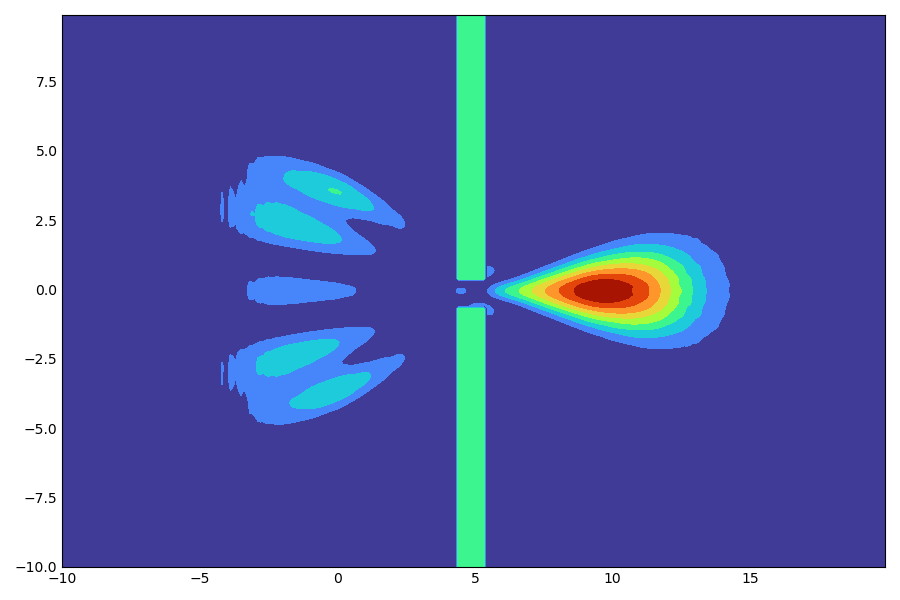
\includegraphics[width=\linewidth]{5/15}
    \end{subfigure}
    \caption{$\Delta y=16\delta,20\delta,30\delta$,t=1100}
\end{figure*}
\onecolumn
\section{Code}
\nolinenumbers
\lstinputlisting[caption=Propagation, language=c]{main.cpp}
\linenumbers
\nolinenumbers
\lstinputlisting[caption=Plot, language=c]{plot.py}
\linenumbers

